
\documentclass[letterpaper,hide notes,xcolor={table,svgnames},pdftex,10pt]{beamer}
\def\showexamples{t}

\usecolortheme{crane}
\setbeamertemplate{navigation symbols}{}

\usetheme{MyPittsburgh}
\usepackage{hyperref}
\usepackage{graphicx,xspace}
\usepackage[normalem]{ulem}
\usepackage{multicol}
\usepackage{amsmath,amssymb,amsthm,graphicx,xspace}
\newcommand\SF[1]{$\bigstar$\footnote{SF: #1}}

\usepackage[sfdefault,lf]{carlito}
\usepackage[T1]{fontenc}
\usepackage[scaled]{beramono}
\usepackage{tikzpagenodes}
\newcommand{\Rplus}{\protect\hspace{-.1em}\protect\raisebox{.35ex}{\small{\small\textbf{+}}}}
\newcommand{\Cpp}{\mbox{C\Rplus\Rplus}\xspace}

\newcounter{tmpnumSlide}
\newcounter{tmpnumNote}

\newcommand\mnote[1]{%
	\addtocounter{tmpnumSlide}{1}
	\ifdefined\showcues {~\tiny\fbox{\arabic{tmpnumSlide}}}\fi
	\note{\setlength{\parskip}{1ex}\addtocounter{tmpnumNote}{1}\textbf{\Large \arabic{tmpnumNote}:} {#1\par}}}

\newcommand\mmnote[1]{\note{\setlength{\parskip}{1ex}#1\par}}


\newcommand\mquestion[2]{{~\color{red}\fbox{?}}\note{\setlength{\parskip}{1ex}\par{\Large \textbf{?}} #1} \note{\setlength{\parskip}{1ex}\par{\Large \textbf{A}} #2\par}\ifdefined \presentationonly \pause \fi}

\newcommand\blackboard[1]{%
	\ifdefined   \showblackboard
		{#1}
	\else {\begin{center} \fbox{\colorbox{blue!30}{%
						\begin{minipage}{.95\linewidth}%
							\hspace{\stretch{1}} Some space intentionally left blank; done at the blackboard.%
						\end{minipage}}}\end{center}}%
	\fi%
}

\usepackage{listings}
\lstset{%
	keywordstyle=\bfseries,
	aboveskip=15pt,
	belowskip=15pt,
	captionpos=b,
	identifierstyle=\ttfamily,
	frame=lines,
	numbers=left, basicstyle=\scriptsize, numberstyle=\tiny, stepnumber=0, numbersep=2pt}

\usepackage{siunitx}
\newcommand\sius[1]{\num[group-separator = {,}]{#1}\si{\micro\second}}
\newcommand\sims[1]{\num[group-separator = {,}]{#1}\si{\milli\second}}
\newcommand\sins[1]{\num[group-separator = {,}]{#1}\si{\nano\second}}
\sisetup{group-separator = {,}, group-digits = true}

%% -------------------- tikz --------------------
\usepackage{tikz}
\usetikzlibrary{positioning}
\usetikzlibrary{arrows,backgrounds,automata,decorations.shapes,decorations.pathmorphing,decorations.markings,decorations.text}

\tikzstyle{place}=[circle,draw=blue!50,fill=blue!20,thick, inner sep=0pt,minimum size=6mm]
\tikzstyle{transition}=[rectangle,draw=black!50,fill=black!20,thick, inner sep=0pt,minimum size=4mm]

\tikzstyle{block}=[rectangle,draw=black, thick, inner sep=5pt]
\tikzstyle{bullet}=[circle,draw=black, fill=black, thin, inner sep=2pt]

\tikzstyle{pre}=[<-,shorten <=1pt,>=stealth',semithick]
\tikzstyle{post}=[->,shorten >=1pt,>=stealth',semithick]
\tikzstyle{bi}=[<->,shorten >=1pt,shorten <=1pt, >=stealth',semithick]

\tikzstyle{mut}=[-,>=stealth',semithick]

\tikzstyle{treereset}=[dashed,->, shorten >=1pt,>=stealth',thin]

\usepackage{ifmtarg}
\usepackage{xifthen}
\makeatletter
% new counter to now which frame it is within the sequence
\newcounter{multiframecounter}
% initialize buffer for previously used frame title
\gdef\lastframetitle{\textit{undefined}}
% new environment for a multi-frame
\newenvironment{multiframe}[1][]{%
	\ifthenelse{\isempty{#1}}{%
		% if no frame title was set via optional parameter,
		% only increase sequence counter by 1
		\addtocounter{multiframecounter}{1}%
	}{%
		% new frame title has been provided, thus
		% reset sequence counter to 1 and buffer frame title for later use
		\setcounter{multiframecounter}{1}%
		\gdef\lastframetitle{#1}%
	}%
	% start conventional frame environment and
	% automatically set frame title followed by sequence counter
	\begin{frame}%
		\frametitle{\lastframetitle~{\normalfont(\arabic{multiframecounter})}}%
		}{%
	\end{frame}%
}
\makeatother

\makeatletter
\newdimen\tu@tmpa%
\newdimen\ydiffl%
\newdimen\xdiffl%
\newcommand\ydiff[2]{%
	\coordinate (tmpnamea) at (#1);%
	\coordinate (tmpnameb) at (#2);%
	\pgfextracty{\tu@tmpa}{\pgfpointanchor{tmpnamea}{center}}%
	\pgfextracty{\ydiffl}{\pgfpointanchor{tmpnameb}{center}}%
	\advance\ydiffl by -\tu@tmpa%
}
\newcommand\xdiff[2]{%
	\coordinate (tmpnamea) at (#1);%
	\coordinate (tmpnameb) at (#2);%
	\pgfextractx{\tu@tmpa}{\pgfpointanchor{tmpnamea}{center}}%
	\pgfextractx{\xdiffl}{\pgfpointanchor{tmpnameb}{center}}%
	\advance\xdiffl by -\tu@tmpa%
}
\makeatother
\newcommand{\copyrightbox}[3][r]{%
	\begin{tikzpicture}%
		\node[inner sep=0pt,minimum size=2em](ciimage){#2};
		\usefont{OT1}{phv}{n}{n}\fontsize{4}{4}\selectfont
		\ydiff{ciimage.south}{ciimage.north}
		\xdiff{ciimage.west}{ciimage.east}
		\ifthenelse{\equal{#1}{r}}{%
			\node[inner sep=0pt,right=1ex of ciimage.south east,anchor=north west,rotate=90]%
			{\raggedleft\color{black!50}\parbox{\the\ydiffl}{\raggedright{}#3}};%
		}{%
			\ifthenelse{\equal{#1}{l}}{%
				\node[inner sep=0pt,right=1ex of ciimage.south west,anchor=south west,rotate=90]%
				{\raggedleft\color{black!50}\parbox{\the\ydiffl}{\raggedright{}#3}};%
			}{%
				\node[inner sep=0pt,below=1ex of ciimage.south west,anchor=north west]%
				{\raggedleft\color{black!50}\parbox{\the\xdiffl}{\raggedright{}#3}};%
			}
		}
	\end{tikzpicture}
}


%% --------------------

%\usepackage[excludeor]{everyhook}
%\PushPreHook{par}{\setbox0=\lastbox\llap{MUH}}\box0}

%\vspace*{\stretch{1}

%\setbox0=\lastbox \llap{\textbullet\enskip}\box0}

\setlength{\parskip}{\fill}

\newcommand\noskips{\setlength{\parskip}{1ex}}
\newcommand\doskips{\setlength{\parskip}{\fill}}

\newcommand\xx{\par\vspace*{\stretch{1}}\par}
\newcommand\xxs{\par\vspace*{2ex}\par}
\newcommand\tuple[1]{\langle #1 \rangle}
\newcommand\code[1]{{\sf \footnotesize #1}}
\newcommand\ex[1]{\uline{Example:} \ifdefined \presentationonly \pause \fi
	\ifdefined\showexamples#1\xspace\else{\uline{\hspace*{2cm}}}\fi}

\newcommand\ceil[1]{\lceil #1 \rceil}


\AtBeginSection[]
{
	\begin{frame}
		\frametitle{Outline}
		\tableofcontents[currentsection]
	\end{frame}
}



\pgfdeclarelayer{edgelayer}
\pgfdeclarelayer{nodelayer}
\pgfsetlayers{edgelayer,nodelayer,main}

\tikzstyle{none}=[inner sep=0pt]
\tikzstyle{rn}=[circle,fill=Red,draw=Black,line width=0.8 pt]
\tikzstyle{gn}=[circle,fill=Lime,draw=Black,line width=0.8 pt]
\tikzstyle{yn}=[circle,fill=Yellow,draw=Black,line width=0.8 pt]
\tikzstyle{empty}=[circle,fill=White,draw=Black]
\tikzstyle{bw} = [rectangle, draw, fill=blue!20,
text width=4em, text centered, rounded corners, minimum height=2em]

\newcommand{\CcNote}[1]{% longname
	This work is licensed under the \textit{Creative Commons #1 3.0 License}.%
}
\newcommand{\CcImageBy}[1]{%
	\includegraphics[scale=#1]{creative_commons/cc_by_30.pdf}%
}
\newcommand{\CcImageSa}[1]{%
	\includegraphics[scale=#1]{creative_commons/cc_sa_30.pdf}%
}
\newcommand{\CcImageNc}[1]{%
	\includegraphics[scale=#1]{creative_commons/cc_nc_30.pdf}%
}
\newcommand{\CcGroupBySa}[2]{% zoom, gap
	\CcImageBy{#1}\hspace*{#2}\CcImageNc{#1}\hspace*{#2}\CcImageSa{#1}%
}
\newcommand{\CcLongnameByNcSa}{Attribution-NonCommercial-ShareAlike}

\newenvironment{changemargin}[1]{% 
	\begin{list}{}{% 
		\setlength{\topsep}{0pt}% 
		\setlength{\leftmargin}{#1}% 
		\setlength{\rightmargin}{1em}
		\setlength{\listparindent}{\parindent}% 
		\setlength{\itemindent}{\parindent}% 
		      \setlength{\parsep}{\parskip}% 
		      }% 
		\item[]}{\end{list}}




\title{Lecture 33 --- File System Implementation}

\author{Jeff Zarnett \\ \small \texttt{jzarnett@uwaterloo.ca}}
\institute{Department of Electrical and Computer Engineering \\
  University of Waterloo}
\date{\today}


\begin{document}

\begin{frame}
  \titlepage

 \end{frame}



\begin{frame}
\frametitle{Implementing the Interface}

Now it is time to go behind the scenes of how the file system lives up to the interface we have just finished discussing. 

The implementation is somewhat complicated, and to keep the size of the problem manageable we will worry about storing files on hard disks.

\begin{center}
	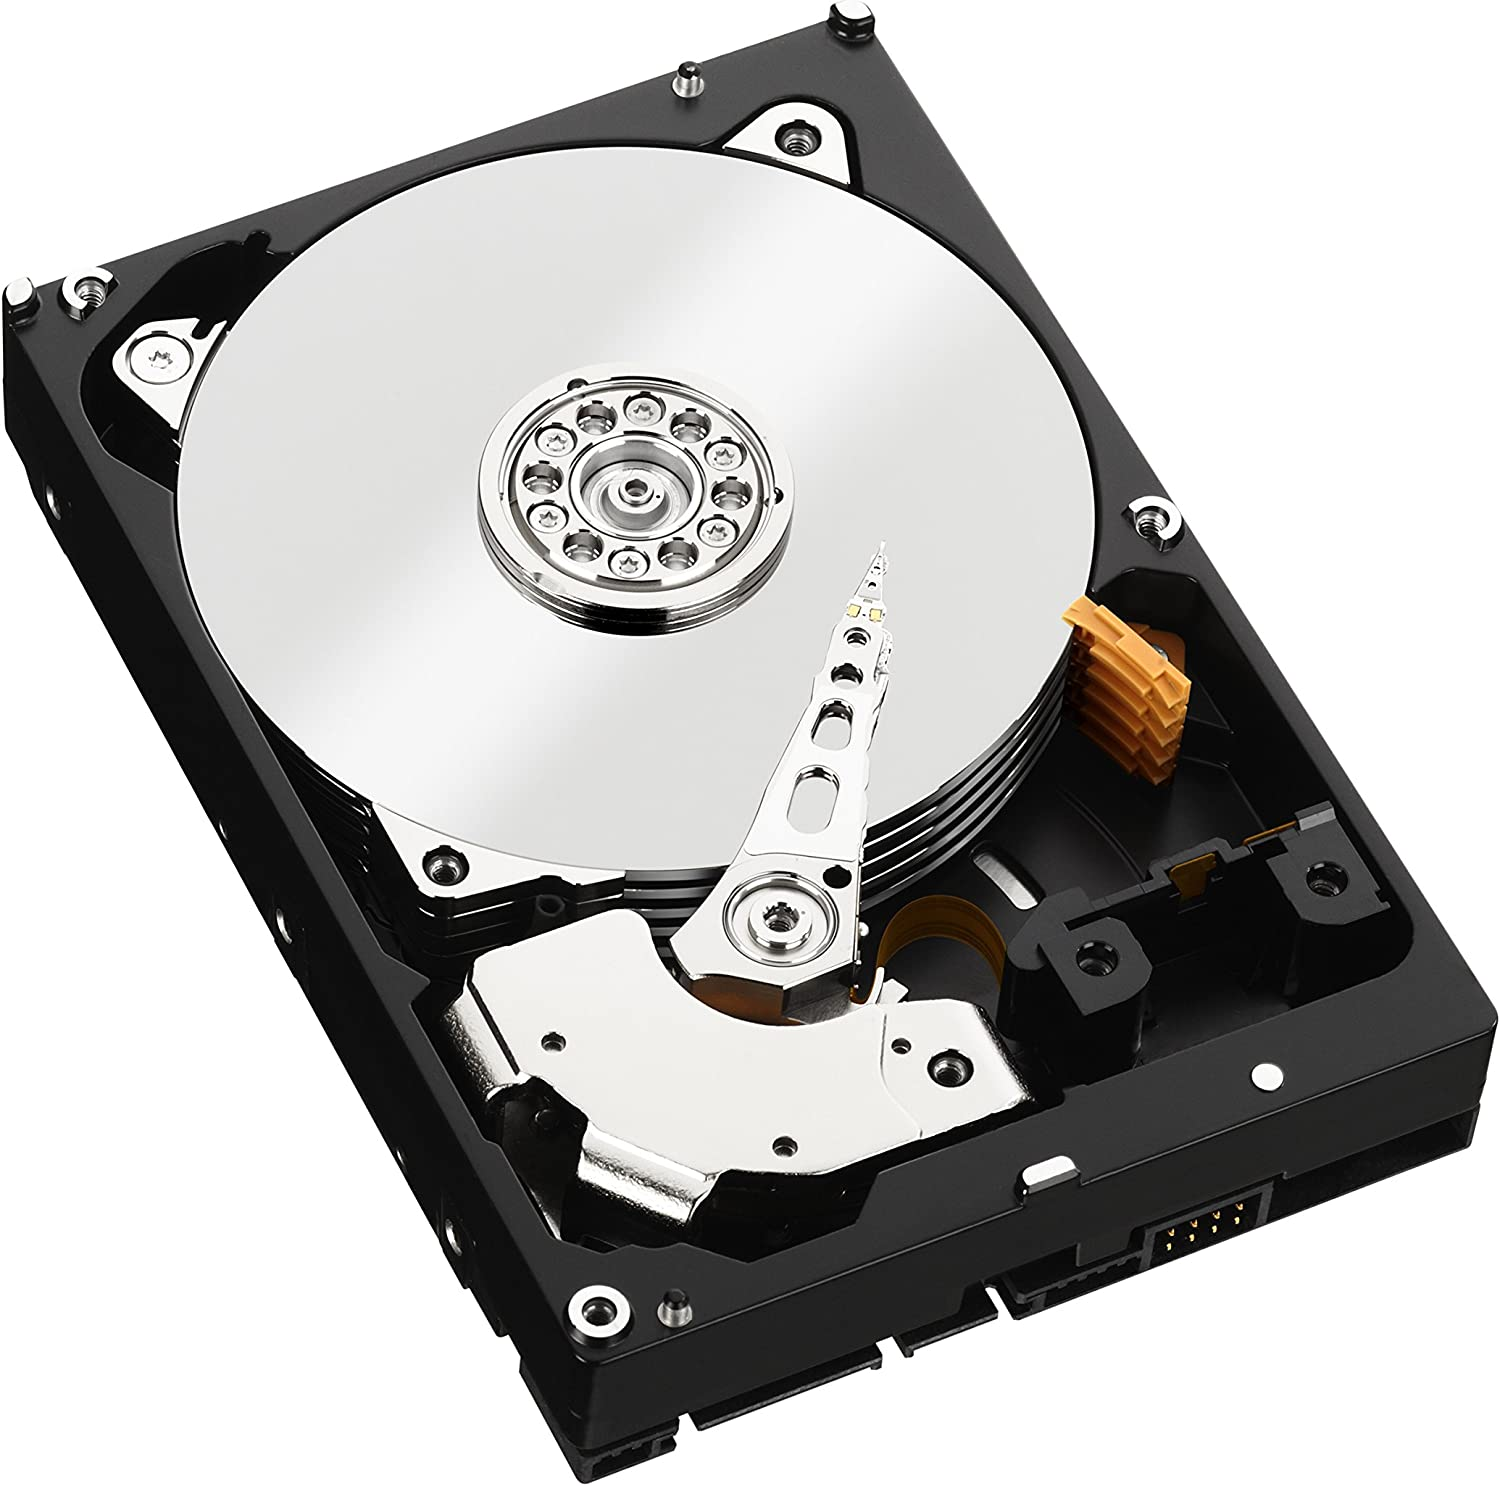
\includegraphics[width=0.35\textwidth]{images/hdd.jpg}
\end{center}

 \end{frame}



\begin{frame}
\frametitle{Implementing the Interface}

 Hard disks themselves make a good choice for this: they are sufficiently large and sufficiently cheap, to start with, to store the data that we want to store. 
 
 We can read an arbitrary part of the disk (unlike a tape). 
 
Finally, we can write to the same part of disk as many times as we want. 
 
Recall also that disks operate on blocks which, in their physical representation, comprise one or more sectors.


\end{frame}

\begin{frame}
\frametitle{Layers of File System Design}

From higher to lower abstraction:

\begin{itemize}
	\item The File System
	\item I/O Control
	\item Basic File System
	\item File Organization Module
	\item Logical File System
\end{itemize}

\end{frame}

\begin{frame}
\frametitle{Disk Organization}

There are a million different file systems (UFS, HFS+, ZFS, NTFS, ext3, FAT32...) 

They are all significantly different, there are some general principles. 

A file system will need to keep track of the total number of blocks, the number and locations of free blocks, the directory structure, and the files themselves.

\end{frame}

\begin{frame}
\frametitle{Disk Organization}

On at least one disk somewhere in the system, there will need to be some information about how to boot up the operating system. 

Not every disk has the operating system on it, but if there is an OS the boot loader is usually put in the first block. 

When the power button is pressed on the case, the BIOS starts up and transfers control to whatever is found at that first block.

\end{frame}

\begin{frame}
\frametitle{Splitting it Up}
Disks may be split, logically, into several different areas, or \alert{partitions}. 

There will be a partition table (sometimes called superblock/master file table).

\end{frame}

\begin{frame}
\frametitle{Splitting it Up}

\begin{center}
	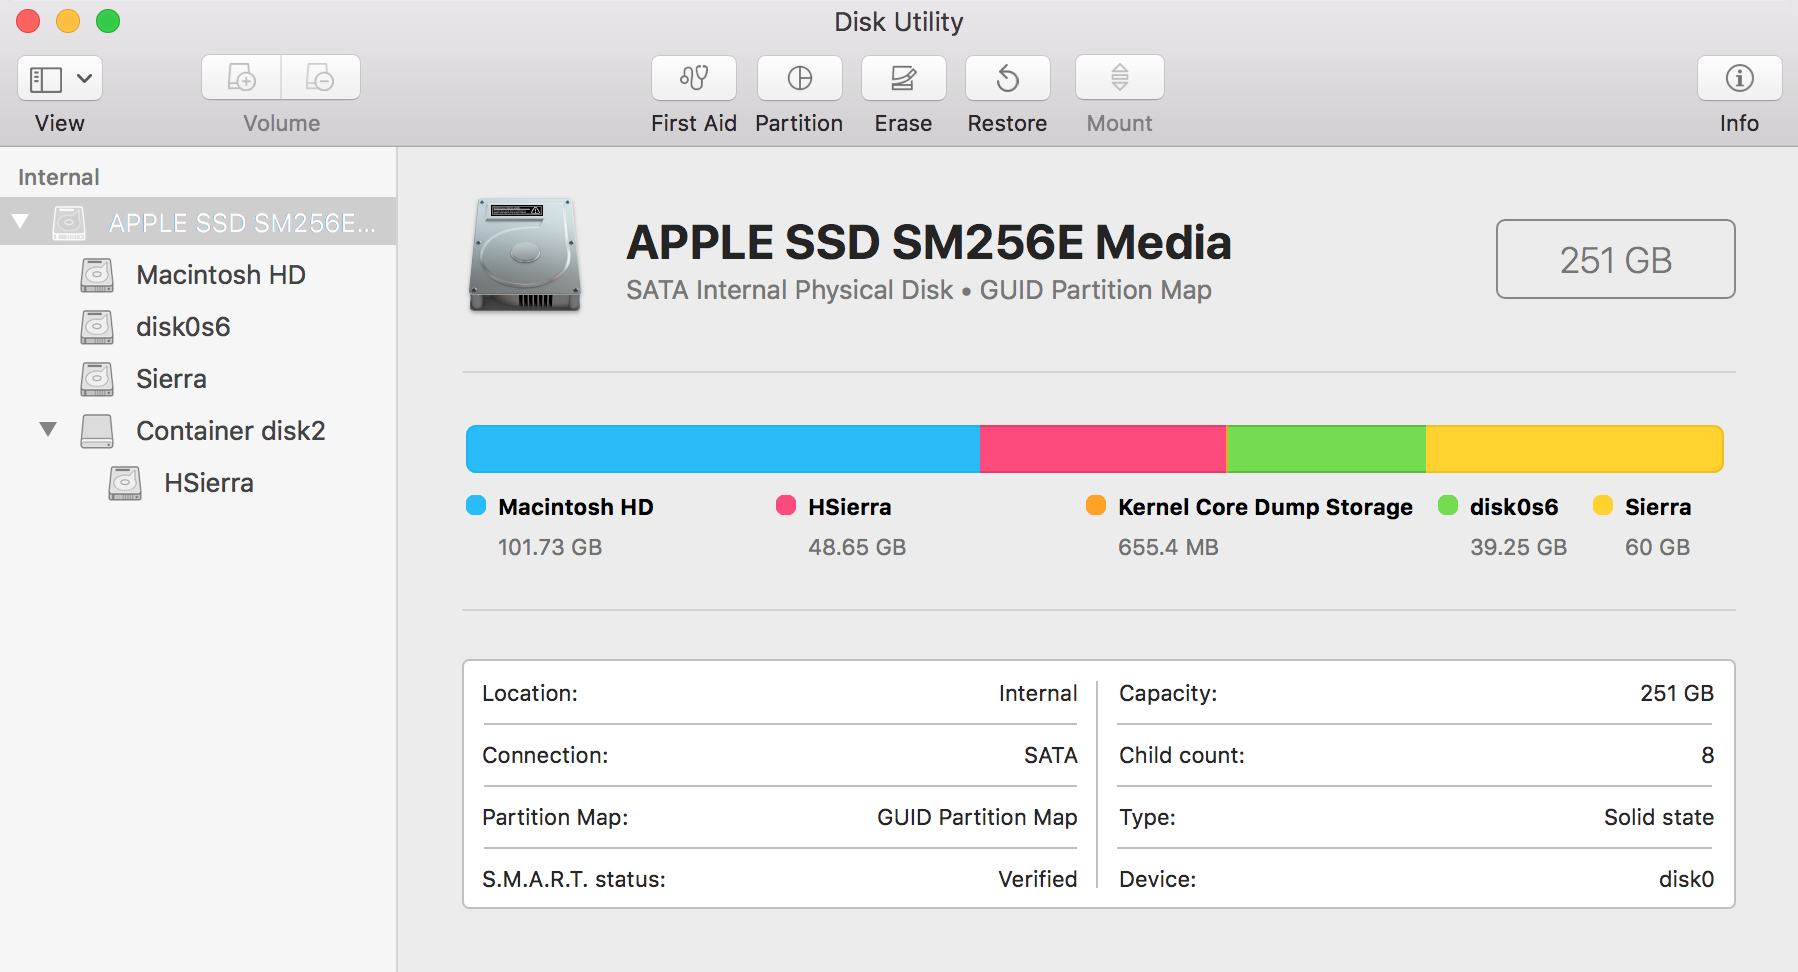
\includegraphics[width=0.75\textwidth]{images/partition-map.png}
\end{center}

In the Windows world we often see the whole disk is in one logical partition (the C: drive, for example, taking the whole primary disk). 

In Linux we often see the disk divided up to have partitions for different things: temporary/swap directory, home directories, boot partition, et cetera...

\end{frame}

\begin{frame}
\frametitle{Caching the File System}

There are several structures that are likely to be in memory for performance reasons:

\begin{enumerate}
	\item \textbf{Mount Table}
	\item \textbf{Cache}
	\item \textbf{Global Open File Table}
	\item \textbf{Process Open File Table}
	\item \textbf{Buffers}
\end{enumerate}

\end{frame}

\begin{frame}
\frametitle{File Control Block}

Creating a new file is the job of the logical file system. 

Allocation of a new FCB (or re-use of an existing free FCB)

\begin{center}
	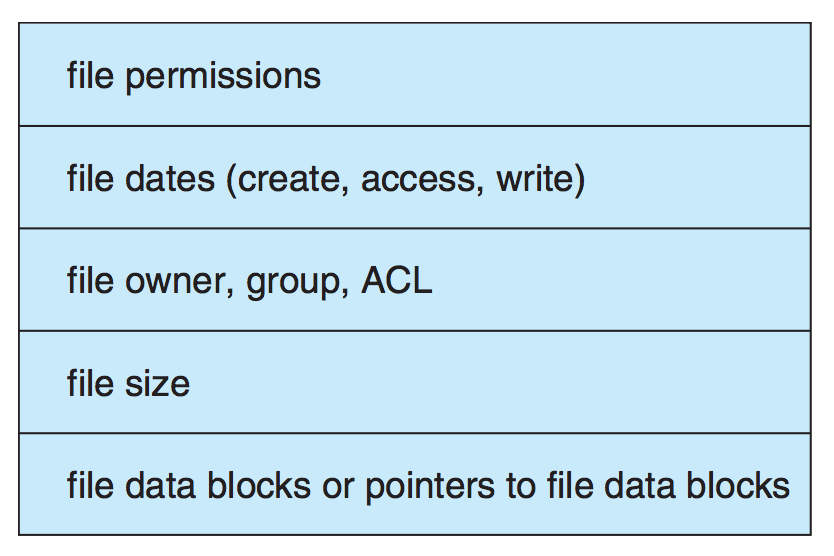
\includegraphics[width=0.4\textwidth]{images/fcb.png}
\end{center}

\end{frame}

\begin{frame}
\frametitle{Opening a File}

If a user (application) actually wants to make use of a file: open system call. 

Open operates on names, the user comprehensible version. 

The file system must then check the global open file table to see if the file is already open somewhere in the system. 

If that file is opened for exclusive access, the open routine returns with an error. 

\end{frame}

\begin{frame}
\frametitle{Opening a File}

If non-exclusive access, then there is no need to search for the file or retrieve it by directory; we just make another reference in the process open file table. 

If the file is not already open, then it needs to be retrieved. 

Once the file is found, the FCB is copied into the global open file table and the appropriate reference is added to the process table.

\end{frame}

\begin{frame}
\frametitle{Opening a File}

The process open file table can contain some additional information, like the next section to read or write, the access mode when the file is open, and so on. 

The open system call returns a pointer to the file table and this is the route through which the application performs all file operations. 

In UNIX this reference is called a \alert{file descriptor}; in Windows a \alert{file handle}.


\end{frame}

\begin{frame}
\frametitle{Closing a File}

The opposite operation to opening a file is obviously to close it. 

When a process closes a file, the entry from the open file table can be removed. 

If this is the last reference to the file a process has, then the file can also be removed from the global open file table. 

Metadata may be updated on close.

\end{frame}



\begin{frame}
\frametitle{Metadata Example: Searching with Spotlight}

An example from Mac OS~X/macOS: the Spotlight system-wide desktop search. 

It was a revelation compared to the previous search options that were slow and did not necessarily include the file content.

\begin{center}
	
\includegraphics[width=0.3\textwidth]{images/sherlock175.jpg}
\end{center}

\end{frame}



\begin{frame}
\frametitle{Metadata Example: Searching with Spotlight}

Spotlight runs queries quickly over the metadata of the system. 

Spotlight examines each file on creation and modification and uses it to update the metadata related to that file. 

Those items are then added to the Spotlight index which can be queried rapidly.

\end{frame}

\begin{frame}
\frametitle{Spotlight Search}

This is a specific case of preparing the data in advance. 

Another example is in exporting data to Excel. 

To export this data, there are two possible ways to do it.

One is to examine and process the data for the Excel file at the time of request. 

The other is to maintain that data separately, and when the Excel report is asked for, take that data and put it in the Excel file.


\end{frame}

\begin{frame}
\frametitle{Maintaining Metadata}

Part of the difficulty with maintaining metadata is when to update it. 

The longer the time between metadata updates, the higher the chance that there will be a user request that gets back out-of-date data. 

The faster the metadata updates, the more time and processing power is spent creating and updating this metadata.


\end{frame}

\begin{frame}
\frametitle{Opening and Reading from a File}

\begin{center}
	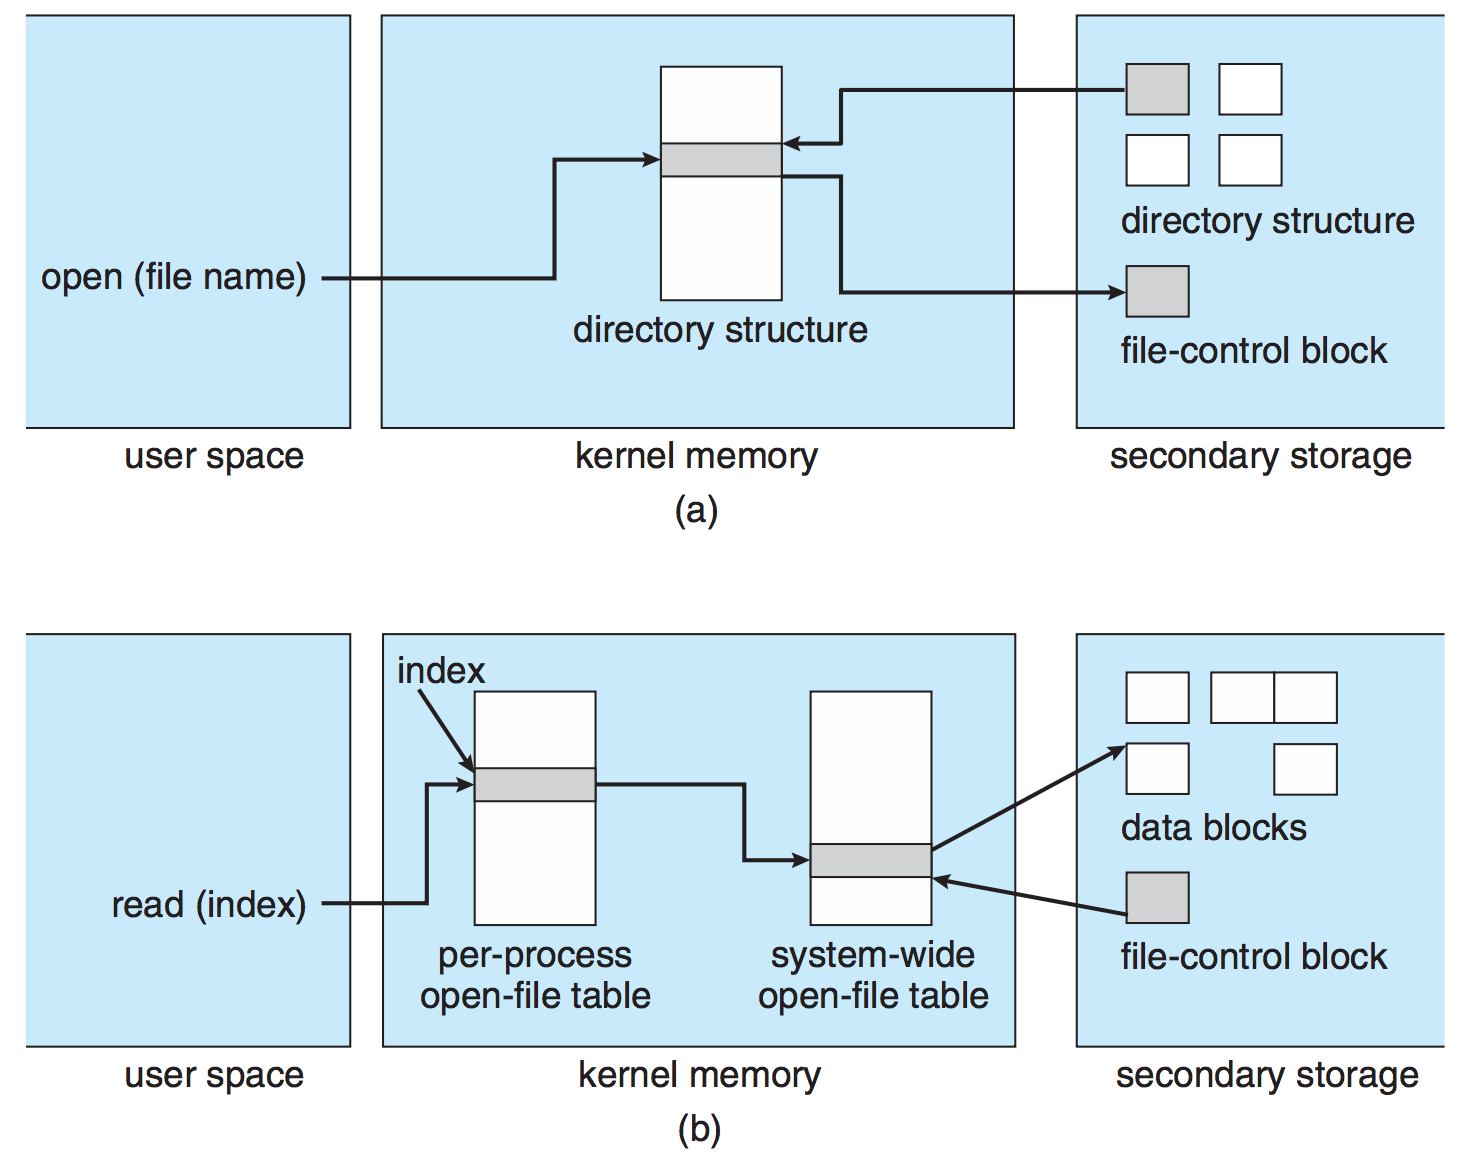
\includegraphics[width=0.75\textwidth]{images/file-system-structures.png}
\end{center}


\end{frame}

\begin{frame}
\frametitle{Virtual File System}

There are a lot of different file systems, like ext3, ZFS... 

These may co-exist in a system, though a partition will be formatted in only one.

From the user's perspective, however, these operate identically. 

This is because of an additional layer of abstraction: virtual file system (VFS). 

\end{frame}

\begin{frame}
\frametitle{Virtual File System}

There are two main purposes to the VFS. 

The first is to separate the file system operations (like reading, writing, opening, and closing files) from the actual implementation. 

Thus operations can be done with whatever file system is implemented. 

The second is that it provides a mechanism for representing a file, uniquely, throughout a network. 

The file representation structure is called a \textit{vnode}, which is rather like an inode, but inodes are unique only within one file system. 

The VFS distinguishes between local and remote files.

\end{frame}

\begin{frame}
\frametitle{Virtual File System}

\begin{center}
	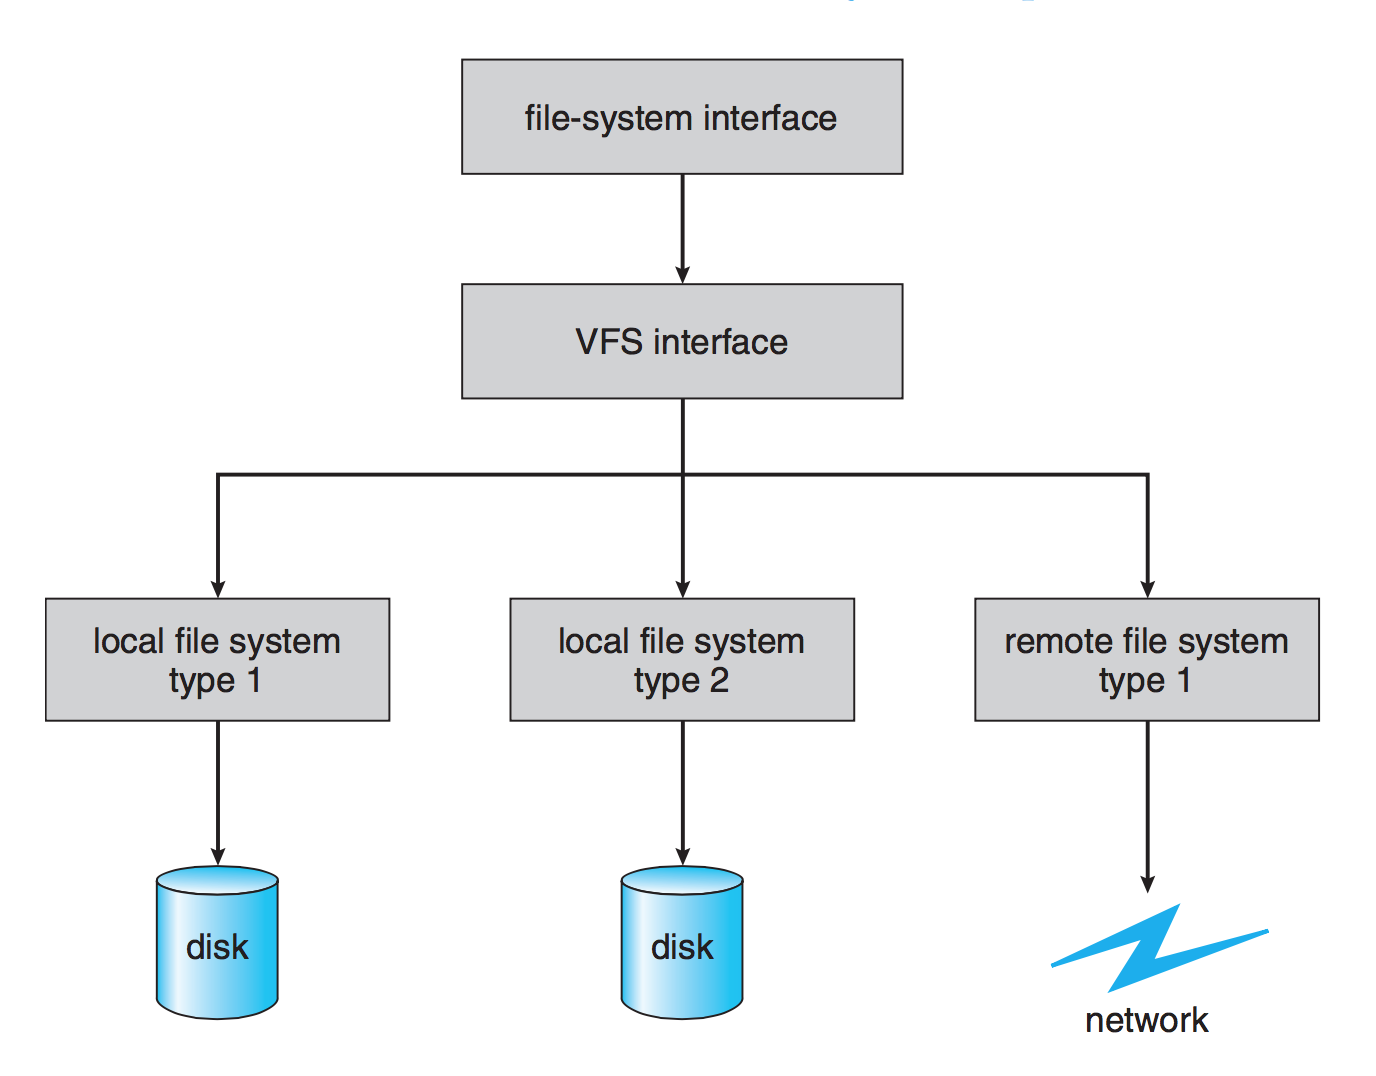
\includegraphics[width=0.85\textwidth]{images/vfs.png}
\end{center}


\end{frame}

\begin{frame}
\frametitle{Virtual File System}

The VFS architecture in Linux has four main objects:

\begin{enumerate}
	\item inode (an individual file)
	\item file (an open file)
	\item superblock (the file system)
	\item dentry (a directory entry)
\end{enumerate}



\end{frame}

\begin{frame}[fragile]
\frametitle{Virtual File System}

For each of those, there are a set of operations defined. 

On a file, for example:
{\scriptsize
\begin{verbatim}
 ssize_t (*read) (struct file *, char __user *, size_t, loff_t *);
 ssize_t (*write) (struct file *, const char __user *, size_t, loff_t *); 
 int (*open) (struct inode *, struct file *);
 int (*flush) (struct file *, fl_owner_t id);
 int (*release) (struct inode *, struct file *);
\end{verbatim}
}

\end{frame}

\begin{frame}
\frametitle{Directory Implementation}

\begin{center}
	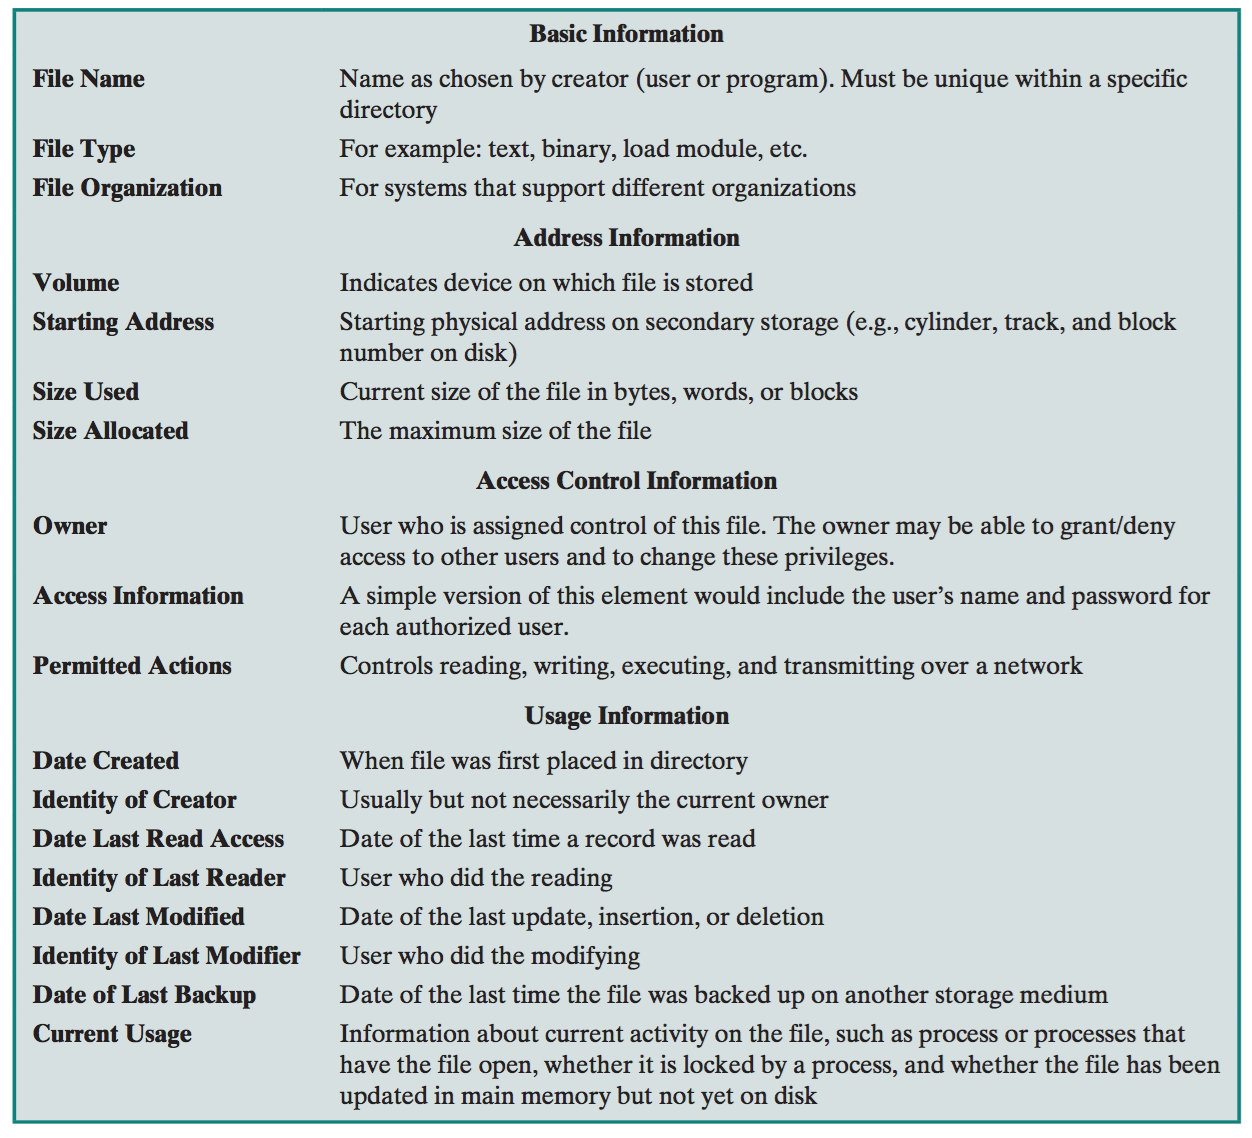
\includegraphics[width=0.75\textwidth]{images/directory.png}
\end{center}

\end{frame}



\begin{frame}
\frametitle{Directory Implementation}

A directory is, after all, not much beyond a set of files. 

And yet, there is a choice to be made in implementing them.

A linear list versus a hash table? 

Both concepts should be familiar to you from data structures and algorithms.


\end{frame}

\begin{frame}
\frametitle{Directory Implementation}

The linear list option is certainly the simplest. 

Creating a new file: search the directory to see if there is a matching file name. 

If not, insert that new entry in the list. 

Deletion is also simple: search the list for the matching file and remove it; if it is the last reference to that file, we can free up the space. 

The real disadvantage to linear lists is that searching takes a long time. 

Searching through a directory can take quite a while.

\end{frame}

\begin{frame}
\frametitle{Directory Implementation}

Alternatively, we could use a hash table. 

The hash is computed based on the file name, and of course there will need to be some strategy for dealing with hash collisions. 

Still, neither of these is satisfactory. 

What we really want is a more complex structure: a tree.


\end{frame}

\begin{frame}
\frametitle{AVL and B-Trees}


An AVL tree might be good as a way of storing ordered data. 

It does not match well with the block system of a hard drive. 

Instead, we will examine a B-Tree, a variation on a binary search tree. 


\end{frame}

\begin{frame}
\frametitle{B-Tree}

Each node should occupy one block, so each node can contain a lot of info. 

File \& directory info is linearly ordered, but a block does not need to be full. 

If a leaf node gets full, we can split it into two half-full blocks. 

Keeping the tree balanced means it takes about the same amount of time to find an item wherever it is.


\end{frame}

\begin{frame}
\frametitle{B-Tree Structure}

A B-Tree structure, formally, has the following characteristics:

\begin{enumerate}
	\item The tree is made up of nodes (have children) and leaves (have no children).
	\item Each node contains at least one key identifying a file record, and more than one pointer to child nodes or child leaves.
	\item Each node has some maximum number of keys.
	\item The keys in a node are stored in non-decreasing order.
\end{enumerate}

\end{frame}



\begin{frame}
\frametitle{B-Tree Properties}

Properties of the B-Tree:

\begin{enumerate}
	\item Every node has at most $2d-1$ keys and $2d$ children ($2d$ pointers).
	\item Every node other than the root has at least $d-1$ keys and $d$ pointers. Each internal node except the root is at least half full and has at least $d$ children.
	\item All leaves appear on the same level.
	\item A non-leaf node with $k$ pointers contains $k-1$ keys.
\end{enumerate}

\end{frame}

\begin{frame}
\frametitle{Searching a B-Tree}

To find something in a B-Tree, the general algorithm is fairly simple:

\begin{enumerate}
	\item Start at the root node. 
	\item If the key is in the current node, it is found, and the algorithm terminates.
	\item If the key is less than the smallest key in this node, follow the leftmost pointer; go to step 2.
	\item If the key is greater than the largest key in this node, follow the rightmost pointer; go to step 2.
	\item If the key is between the values of two adjacent keys, follow the pointer between them; go to step 2.
\end{enumerate}



\end{frame}

\begin{frame}
\frametitle{B-Tree Insertion}

Insertion into the B-Tree is more complicated:

\begin{enumerate}
	\item Search the tree for the key. If it is not found, then we are at least looking at the block where it would be if it were there.
	\item If this node has fewer than $2d-1$ keys (that is, it is not full), insert the key into this node in the proper sequence. The algorithm terminates.
	\item If the node is full, split this node around the median key into two new nodes with $d-1$ keys each. Promote the median key to the higher level. If the new node is less than the median key, insert it in the left-hand new node; otherwise into the right.
	\item The promoted node is inserted into the parent node in order, splitting the parent if the parent is already full.
	\item If the process of promotion reaches the root node and the root is full, then splitting and promotion occurs and the height of the tree increases by 1.
\end{enumerate}


\end{frame}



\begin{frame}
\frametitle{B-Tree Operations}


\begin{center}
	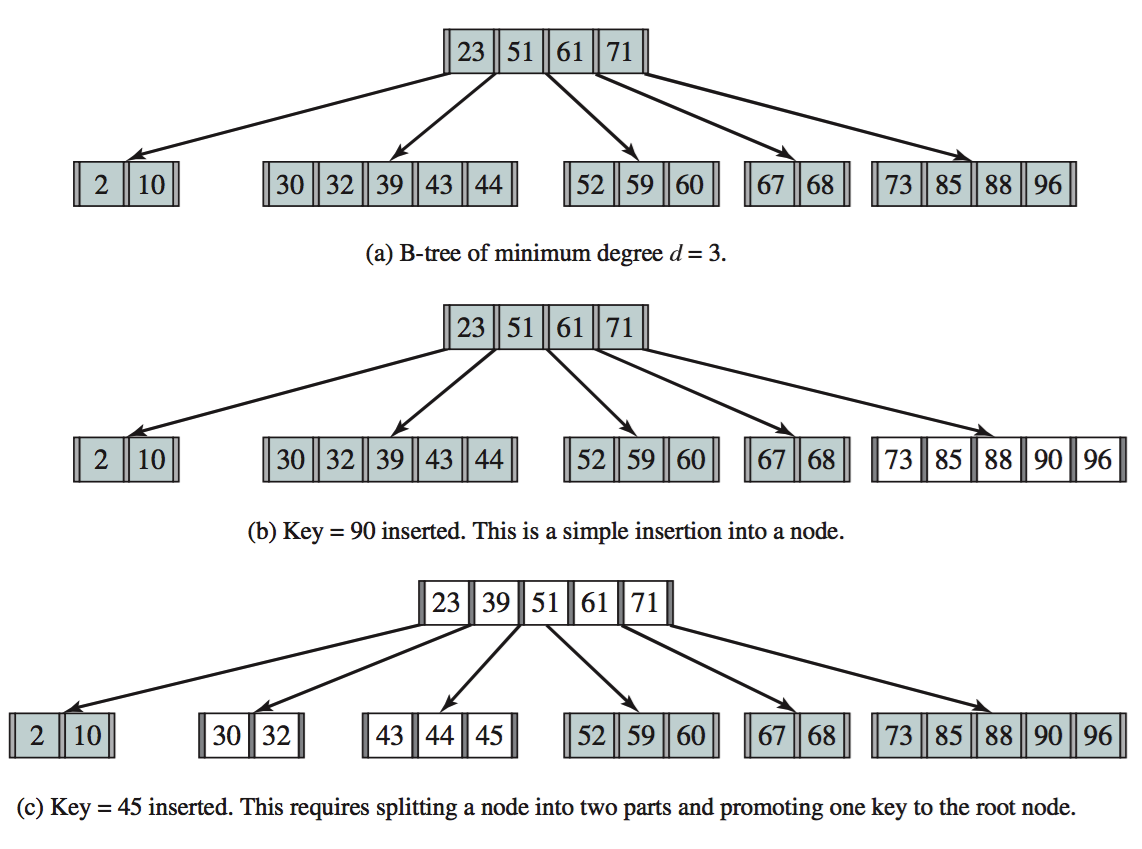
\includegraphics[width=0.9\textwidth]{images/b-tree-insert-top.png}
\end{center}


\end{frame}

\begin{frame}
\frametitle{B-Tree Operations}


\begin{center}
	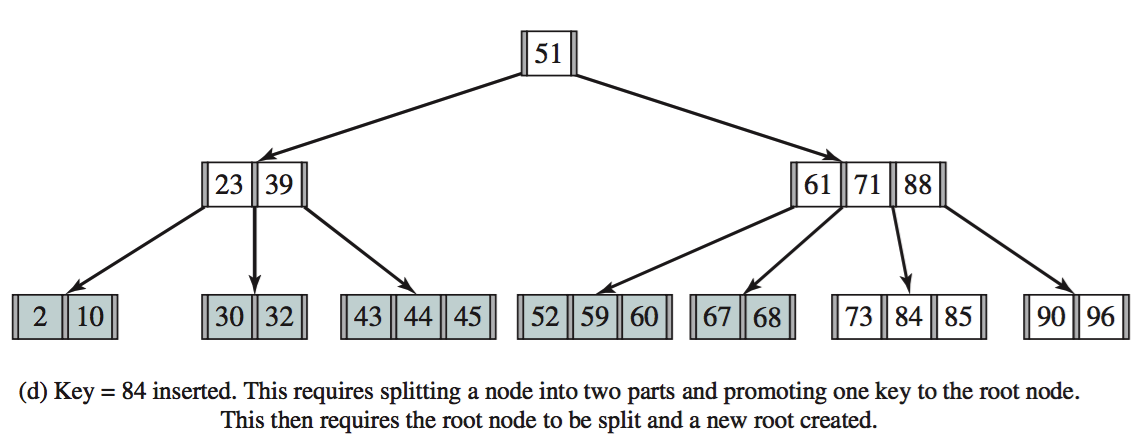
\includegraphics[width=0.9\textwidth]{images/b-tree-insert-bottom.png}
\end{center}


\end{frame}

\end{document}

